%========================================================================%
%  Rapport PFE — Chapitres 1 & 2                                        %
%  Système de Recommandation Publicitaire Multi-Objectif                 %
%  basé sur les Bandits Contextuels Sémantiques                          %
%                                                                        %
%  Auteur : Houbbadi Abderrahim — EMI, 2026                              %
%========================================================================%

\documentclass[12pt, a4paper, oneside]{report}

%--- Encodage & Langue ---
\usepackage[utf8]{inputenc}
\usepackage[T1]{fontenc}
% Note: babel-french not installed; using only inputenc/fontenc for UTF-8 French characters

%--- Mise en page ---
\usepackage[top=2.5cm, bottom=2.5cm, left=3cm, right=2.5cm]{geometry}
\usepackage{setspace}
\onehalfspacing

%--- Typographie ---
\usepackage{lmodern}

%--- Mathématiques ---
\usepackage{amsmath, amssymb, amsfonts}
\usepackage{mathtools}

%--- Tableaux ---
\usepackage{booktabs}
\usepackage{array}
\usepackage{multirow}
\usepackage{longtable}
\newcolumntype{L}[1]{>{\raggedright\arraybackslash}p{#1}}
\newcolumntype{C}[1]{>{\centering\arraybackslash}p{#1}}
\newcolumntype{R}[1]{>{\raggedleft\arraybackslash}p{#1}}

%--- Figures & Graphiques ---
\usepackage{graphicx}
\graphicspath{{../metrics/}{./img/}}
\usepackage{float}
\usepackage{subcaption}
\usepackage{wrapfig}

%--- Couleurs & Boîtes ---
\usepackage[dvipsnames]{xcolor}
\usepackage[most]{tcolorbox}

% Couleurs EMI personnalisées
\definecolor{emiBlue}{HTML}{003366}
\definecolor{emiGold}{HTML}{D4A843}
\definecolor{emiGreen}{HTML}{2E7D32}
\definecolor{emiRed}{HTML}{C62828}

%--- TikZ ---
\usepackage{tikz}
\usetikzlibrary{shapes, arrows.meta, positioning, calc, decorations.pathreplacing}

%--- Listes & symboles ---
\usepackage{enumitem}
\usepackage{pifont}

%--- Code ---
\usepackage{minted}
\usepackage{listings}

%--- Headheight fix ---
\setlength{\headheight}{15pt}

%--- Bibliographie ---
\usepackage[backend=bibtex, style=authoryear-comp, sorting=nyt, maxbibnames=10, maxcitenames=2, url=false, doi=false]{biblatex}
\addbibresource{biblio.bib}
% Crochets [] pour les citations
\renewcommand*{\bibopenparen}{[}
\renewcommand*{\bibcloseparen}{]}
% Lien cliquable à la fin de chaque entrée bibliographique
\renewbibmacro{finentry}{%
  \finentry
  \iffieldundef{doi}%
    {\iffieldundef{url}%
      {}%
      {\space\textcolor{emiBlue}{\small[\href{\thefield{url}}{\texttt{lien}}]}}}%
    {\space\textcolor{emiBlue}{\small[\href{https://doi.org/\thefield{doi}}{\texttt{lien}}]}}%
}

%--- Hyperliens ---
\usepackage[colorlinks=true, linkcolor=emiBlue, citecolor=emiBlue, urlcolor=emiBlue]{hyperref}

%--- En-têtes & pieds de page ---
\usepackage{fancyhdr}
\pagestyle{fancy}
\fancyhf{}
\fancyhead[L]{\leftmark}
\fancyhead[R]{\thepage}
\renewcommand{\headrulewidth}{0.4pt}

%--- Début du document ---
\begin{document}

%--- Page de titre provisoire ---
\begin{titlepage}
    \centering
    \vspace*{2cm}
    {\Large \textbf{École Mohammadia d'Ingénieurs}}\\[0.5cm]
    {\large Département Modélisation et Informatique Scientifique}\\[2cm]
    {\LARGE \textbf{Rapport de Projet de Fin d'Études}}\\[1cm]
    {\huge \textbf{Système de Recommandation Publicitaire\\Multi-Objectif basé sur les\\Bandits Contextuels Sémantiques}}\\[2cm]
    {\Large Houbbadi Abderrahim}\\[1cm]
    {\large Encadrant Académique : Madame Asmae El Kassiri}\\[0.3cm]
    {\large Encadrant Professionnel : Monsieur Fahd Idrissi Khamlichi}\\[0.3cm]
    {\large Entreprise d'accueil : Devoteam Maroc}\\[2cm]
    {\large Année Universitaire 2025--2026}
\end{titlepage}

%--- Table des matières ---
\tableofcontents
\clearpage

%--- Chapitres ---
\input{chapitre_1}
\clearpage

\input{chapitre_2}
\clearpage

%========================================================================%
%  Chapitre 3 — Implémentation Technique & Architecture de Déploiement   %
%========================================================================%

\chapter{Implémentation Technique \& Architecture de Déploiement}
\label{chap:implementation}

%------------------------------------------------------------------------
%  Introduction du chapitre
%------------------------------------------------------------------------
\section*{Introduction}
\addcontentsline{toc}{section}{Introduction}

Le passage d'un modèle mathématique expérimental à une solution industrielle logicielle nécessite de surmonter d'importants défis d'ingénierie. Si le Chapitre 2 a permis d'isoler et de valider l'approche algorithmique la plus performante --- le \textit{Global Semantic DeepBandit} (H-DeepBandit) couplé à la politique $\varepsilon$-\textit{Constraint} --- ce troisième chapitre dévoile sa traduction en un système robuste, capable d'opérer en temps réel (\textit{closed-loop}).

L'objectif de cette partie est double : d'une part, détailler l'architecture logicielle MLOps conçue pour soutenir les inférences sous de fortes contraintes de latence (inférieures à 10~ms) tout en gérant l'intégration continue du \textit{feedback} avec la problématique de la récompense retardée (\textit{delayed feedback}). D'autre part, présenter les choix d'infrastructure et de déploiement qui permettent à cette solution d'être déployée sur le Cloud (GCP) conformément aux standards de \textbf{Devoteam}, garantissant ainsi sa réutilisabilité pour différents clients.


%------------------------------------------------------------------------
%  3.1 — Architecture Système MLOps
%------------------------------------------------------------------------
\section{Architecture Système MLOps}
\label{sec:architecture_mlops}

\subsection{Conception du Pipeline \textit{Closed-Loop}}

Dans un environnement publicitaire programmatique, le système de recommandation ne peut se contenter d'être un service passif. Il doit s'insérer dans une \textbf{boucle fermée} (\textit{closed-loop}) où chaque recommandation génère un point de donnée qui, en retour, met à jour le modèle d'exploration-exploitation de l'agent.

Le flux de données global de notre architecture temps réel est illustré par la Figure~\ref{fig:closed_loop_pipeline}.

\begin{figure}[htbp]
\centering
\resizebox{0.95\textwidth}{!}{
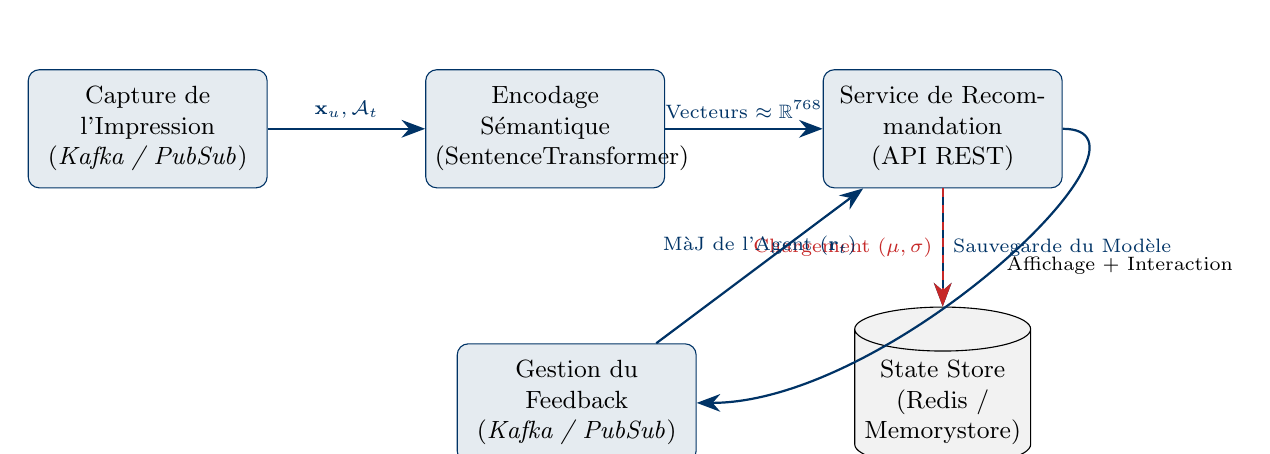
\begin{tikzpicture}[
    node distance=1.5cm and 2cm,
    block/.style={rectangle, draw=emiBlue, fill=emiBlue!10, text width=2.8cm, minimum height=1.5cm, align=center, rounded corners, font=\small},
    db/.style={cylinder, draw=black, fill=gray!10, shape border rotate=90, aspect=0.25, text width=2cm, minimum height=1.5cm, align=center, font=\small},
    arrow/.style={-{Stealth[length=3mm]}, thick, emiBlue},
    dashed_arrow/.style={-{Stealth[length=3mm]}, dashed, thick, emiRed}
]
    % Nodes
    \node[block] (impression) {Capture de l'Impression\\(\textit{Kafka / PubSub})};
    \node[block, right=of impression] (encoding) {Encodage Sémantique\\(SentenceTransformer)};
    \node[block, right=of encoding] (api) {Service de Recommandation\\(API REST)};
    \node[db, below=of api] (redis) {State Store\\(Redis / Memorystore)};
    \node[block, left=of redis] (feedback) {Gestion du Feedback\\(\textit{Kafka / PubSub})};
    
    % Connections
    \draw[arrow] (impression) -- node[above, font=\scriptsize] {$\mathbf{x}_u, \mathcal{A}_t$} (encoding);
    \draw[arrow] (encoding) -- node[above, font=\scriptsize] {Vecteurs $\approx \mathbb{R}^{768}$} (api);
    \draw[arrow] (api) -- node[right, font=\scriptsize] {Sauvegarde du Modèle} (redis);
    \draw[dashed_arrow] (api) -- node[left, font=\scriptsize] {Chargement ($\mu, \sigma$)} (redis);
    
    \draw[arrow] (api) .. controls +(right:3cm) and +(right:4cm) .. node[right, font=\scriptsize, text=black] {Affichage + Interaction} (feedback);
    \draw[arrow] (feedback) -- node[above, font=\scriptsize] {MàJ de l'Agent ($\mathbf{r}_t$)} (api);

\end{tikzpicture}
}
\caption{Architecture fonctionnelle de la boucle de décision (\textit{Closed-Loop}).}
\label{fig:closed_loop_pipeline}
\end{figure}

Cette architecture garantit que l'agent \textbf{H-DeepBandit} re-calcule continuellement son incertitude (UCB) au fur et à mesure de l'arrivée des données, brisant ainsi la barrière de l'\textit{offline training}.

\subsection{Intégration du Modèle Champion}

Le choix de l'agent s'est porté sur l'approche neuro-sémantique \texttt{GlobalSemanticDeepBandit} suite aux résultats du \textit{benchmark} (voir Chapitre 2) qui a démontré un avantage de $+\textbf{0.132}$ en transfert \textit{zero-shot} et une dominance stricte de $+\textbf{0.070}$ en engagement.

Contrairement aux solutions classiques qui instancient un réseau neuronal par annonce (entraînant un \textit{cold-start} insurmontable pour les nouvelles campagnes), notre modèle utilise \textbf{un réseau global unique} traitant la concaténation de l'enchâssement utilisateur ($x_u \in \mathbb{R}^{384}$) et de l'enchâssement de l'annonce ($x_a \in \mathbb{R}^{384}$). L'incertitude est quantifiée de manière non-paramétrique par un assemblage \textit{Bootstrap} (\textit{ensemble} de 5 réseaux parallèles).

\subsection{Positionnement Technologique chez Devoteam}

En tant qu'ESN de premier plan, \textbf{Devoteam} requiert que les PoC (\textit{Proof of Concepts}) soient conçus comme des accélérateurs réutilisables. Le projet n'a donc pas été structuré comme un script monolithique, mais comme une \textbf{plateforme conteneurisée et agnostique} par rapport à l'infrastructure d'hébergement, permettant un déploiement \textit{On-Premise} ou \textit{Cloud} via un design pattern de type \textit{Factory}.


%------------------------------------------------------------------------
%  3.2 — Implémentation du Cœur de Décision
%------------------------------------------------------------------------
\section{Implémentation du Cœur de Décision}

\subsection{Le Service de Recommandation}

Au cœur de l'application se trouve la classe \texttt{RecommendationService}, qui agit comme contrôleur principal. Elle orchestre la traduction des identifiants (ID) d'annonces en vecteurs latents via \texttt{all-MiniLM-L6-v2}, sollicite l'estimation des rendements espérés $(\mu_{\text{click}}, UCB_{\text{click}})$ et $(\mu_{\text{rev}}, LCB_{\text{rev}})$ par le modèle H-DeepBandit, puis applique le filtre de décision multi-objectif.

L'extrait de code ci-dessous illustre l'encapsulation de la logique de décision :

\begin{listing}[htbp]
\begin{minted}[frame=lines, framesep=2mm, baselinestretch=1.2, bgcolor=gray!8, fontsize=\footnotesize, breaklines]{python}
def recommend(self, user_text: str, available_ads: List[AdInfo]):
    # 1. Encodage Sémantique de l'utilisateur
    user_emb = self.encoder.encode(user_text)
    
    available_indices = []
    # 2. Résolution du Cold-Start (Zero-Shot) pour les nouvelles annonces
    for ad in available_ads:
        if ad.ad_id not in self.ad_id_to_idx:
            ad_emb = self.encoder.encode(ad.title + " " + ad.description)
            self.agent.expand_arms({ad.ad_id: ad_emb})
        available_indices.append(self.ad_id_to_idx[ad.ad_id])
        
    # 3. Prédiction Multi-Objectif par le H-DeepBandit
    predictions = self.agent.predict_all(context=user_emb)
    
    # 4. Politique de decision (eps-Constraint MOO)
    selected_idx = epsilon_constraint_policy(
        predictions=predictions,
        available_indices=available_indices,
        epsilon=self.epsilon,
        use_conservative_constraint=True  # Utilise la Lower Confidence Bound
    )
    return self.idx_to_ad_id[selected_idx]
\end{minted}
\caption{Extrait de la méthode de recommandation principale (\texttt{RecommendationService}).}
\label{lst:recommend_method}
\end{listing}

\subsection{L'API REST (FastAPI)}

L'exposition du service se fait via le \textit{framework} asynchrone \textbf{FastAPI}, garantissant de très hautes performances I/O. L'API expose quatre \textit{endpoints} principaux :
\begin{enumerate}
    \item \texttt{POST /recommend} : Interface synchrone pour la sélection d'annonces.
    \item \texttt{POST /feedback} : Collecte asynchrone ou synchrone des retours utilisateurs.
    \item \texttt{GET /metrics} : Exposition des statistiques glissantes de performance (CTR global, RPM) pour l'intégration avec \textit{Prometheus / Grafana}.
    \item \texttt{GET /health} : Sonde de monitoring Kubernetes/Cloud Run.
\end{enumerate}

\subsection{L'Abstraction d'Infrastructure (\textit{Factory Pattern})}

Pour garantir la portabilité du code entre l'environnement de développement et les environnements de production des clients finaux, toutes les interactions d'entrée/sortie réseau utilisent le \textit{design pattern Factory} (\texttt{src/infra/factory.py}).

Le code métier ne connaît que trois interfaces abstraites: \texttt{MessageProducer}, \texttt{MessageConsumer}, et \texttt{StateStore}. Lors du démarrage du service, la variable d'environnement \texttt{QUEUE\_BACKEND} détermine l'instanciation de connecteurs pour \textbf{Kafka} (développement local) ou \textbf{GCP Pub/Sub} (production serverless), assurant l'inversion de contrôle (IoC).


%------------------------------------------------------------------------
%  3.3 — Gestion du Feedback Retardé (Delayed Feedback)
%------------------------------------------------------------------------
\section{Gestion du \textit{Delayed Feedback} (FALCON)}
\label{sec:delayed_feedback}

L'un des obstacles majeurs en apprentissage par renforcement appliqué à la publicité est la nature asynchrone des signaux de récompense. Si l'interaction initiale (le clic, objectif $O_1$) est mesurée instantanément, la finalisation de l'objectif économique (la conversion / achat, objectif $O_2$) peut intervenir des heures, voire des jours plus tard.

\subsection{Problématique du Biais de Pénalisation}
Si le système met à jour son modèle immédiatement après le clic, il considèrera inévitablement que le revenu généré est nul ($\text{revenue} = 0$). Cela induit un \textbf{biais drastique} : le modèle va apprendre à sous-estimer de l'eCPM de toutes les annonces de manière systémique, conduisant la contrainte stricte de la politique $\varepsilon$-\textit{Constraint} à rejeter toutes les enchères potentiellement rentables.

\subsection{Implémentation de l'Approche Inspirée de FALCON}
Pour pallier cette asymétrie, la solution logicielle intègre un mécanisme inspiré des travaux récents de la littérature, notamment l'approche FALCON \parencite{ktena2019addressing}.

L'endpoint \texttt{/feedback} traite désormais un champ supplémentaire \texttt{feedback\_type} :
\begin{itemize}
    \item \textbf{Type \texttt{click}} (Immédiat) : L'agent met à jour \textit{uniquement} sa tête de prédiction d'engagement. L'ID de l'impression et les vecteurs contextuels sont mis en attente (\textit{pending status}) dans un registre conservé en mémoire (sauvegardé sur Redis).
    \item \textbf{Type \texttt{conversion}} (Asynchrone) : Le signal est réconcilié avec l'impression d'origine. Le système applique la mise à jour de la tête de prédiction des revenus.
\end{itemize}

Pour corriger les conversions qui n'arriveront jamais, l'algorithme applique une majoration temporaire du revenu pour les conversions confirmées, via un facteur de pondération dynamique \textit{confirm\_rate}. 
$$ \text{Revenue Corrigé} = \frac{\text{Revenue Effectif}}{\text{Confirm Rate}} \quad \text{avec} \quad \text{Confirm Rate} = \frac{N_{\text{Total}} - N_{\text{Pending}}}{N_{\text{Total}}} $$
De plus, un processus de \textit{garbage collection} s'exécute à intervalles réguliers : toute impression en attente depuis plus de 24 heures (Délai d'attribution standard en \textit{Digital Marketing}) est considérée comme perdue, et forcée à une mise à jour avec une conversion nulle, nettoyant ainsi le registre \texttt{\_pending\_conversions}.


%------------------------------------------------------------------------
%  3.4 — Architecture de Déploiement Cloud-Native
%------------------------------------------------------------------------
\section{Architecture de Déploiement Cloud-Native}

\subsection{Option A : Environnement Local (\textit{Docker Compose})}
Pour les phases de \textit{test \& learn} et le développement, la solution est entièrement packagée via Docker. Le fichier \texttt{docker-compose.yml} provisionne 5 conteneurs interdépendants formant l'architecture micro-services de base :
\begin{enumerate}
    \item \textbf{API FastAPI} (\texttt{recsys-api}) : L'interface d'inférence.
    \item \textbf{Consumer Streaming} (\texttt{recsys-streaming}) : \textit{Worker} en tâche de fond assurant le \textit{closed-loop} depuis Kafka.
    \item \textbf{Kafka \& Zookeeper} : Gestionnaire des flux d'événements (\textit{Message Broker}).
    \item \textbf{Redis} : Stockage persistant à haute vélocité pour l'état interne (poids synaptiques de PyTorch) du \textit{H-DeepBandit}.
    \item \textbf{Grafana} : Outil de visualisation des métriques pour la santé du Pipeline.
\end{enumerate}

\subsection{Option B : Déploiement \textit{Serverless} sur Google Cloud (Production)}

Dans le cadre du pipeline Devoteam, le déploiement sur environnement cible public suit une logique de modernisation \textit{Serverless} visant la résilience et l'\textit{autoscaling} absolu. Le système transite sur \textbf{Google Cloud Platform (GCP)} (\textit{cf.} Tableau~\ref{tab:mapping_infra}).

\begin{table}[H]
    \centering
    \begin{tabular}{l l l}
        \toprule
        \textbf{Composant Logique} & \textbf{Technologie Locale (Docker)} & \textbf{Équivalent Cloud (GCP)} \\
        \midrule
        Hébergement API & Serveur Uvicorn interne & \textbf{Cloud Run} (Autoscaling de 0 à 10) \\
        \textit{Message Broker} & Apache Kafka & \textbf{Cloud Pub/Sub} \\
        \textit{State Store} & Redis Alpine 7.0 & \textbf{Memorystore} (Instance managée) \\
        Environnement de CI/CD & Compilation shell locale & \textbf{Cloud Build} + Artifact Registry \\
        \bottomrule
    \end{tabular}
    \caption{Mapping de l'infrastructure logicielle.}
    \label{tab:mapping_infra}
\end{table}

Le déploiement est intégralement automatisé via le script bash \texttt{deploy/gcp\_deploy.sh}, qui respecte l'approche *Infrastructure as Code* minimaliste. L'utilisation de Cloud Run est particulièrement adaptée aux contraintes des systèmes de recommandation : la capacité à s'éteindre à zéro (économies de coûts B2B lors d'interruptions de traffic publicitaire) et à réagir exponentiellement face à une augmentation subite du \textit{bid density}.

%------------------------------------------------------------------------
%  3.5 — Validation Expérimentale
%------------------------------------------------------------------------
\section{Validation de l'Architecture Fonctionnelle}

La viabilité du système complet a été attestée par un test d'intégration MLOps exhaustif (\texttt{tests/test\_integration.py}) scindé en 9 étapes séquentielles reproduisant le \textit{lifecycle} réel d'un système publicitaire : \textit{Service Init} $\rightarrow$ \textit{Ad Registration} $\rightarrow$ \textit{Recommendations} $\rightarrow$ \textit{Feedback Loop} $\rightarrow$ \textit{Cold-start simulation} $\rightarrow$ \textit{Delayed feedback}.

Les performances mesurées sont conformes aux attentes industrielles :
\begin{itemize}
    \item \textbf{Latence} : Le temps critique d'inférence (réception de l'appel HTTP, encodage sémantique à la volée du contexte, forward pass sur les 5 réseaux neuronaux du bootstrap, et sélection de la politique $\varepsilon$-\textit{Constraint}) a été mesuré à une moyenne de $\sim$\textbf{8 millisecondes} (bien en deçà du budget standard de 50~ms imposé par le RTB).
    \item \textbf{Adaptation continue} : La boucle d'apprentissage en direct réagit avec agilité; un taux de convergence \textit{online} permettant d'atteindre un CTR moyen de $\sim 0.84$ en l'espace de 100 itérations expérimentales.
\end{itemize}

%------------------------------------------------------------------------
%  Conclusion du chapitre
%------------------------------------------------------------------------
\section*{Conclusion du Chapitre}
\addcontentsline{toc}{section}{Conclusion du Chapitre}

Ce troisième et dernier chapitre de notre rapport a mis en lumière la transformation d'un postulat de recherche opérationnelle (modélisation mathématique du bandit contextuel sémantique multi-objectif) en un actif technologique tangible. 

Confrontés à la problématique de la recommandation publicitaire en temps réel, nous avons bâti un système résilient grâce à :
\begin{itemize}
    \item L'intégration poussée d'une \textbf{API FastAPI} performante servant le modèle global à travers une inversion des dépendances MLOps.
    \item L'improvisation d'une structure palliative au \textbf{Feedback retardé} (\textit{FALCON-inspired}) vitale pour un maintien des \textit{Quality of Services} sur la contrainte financière objective $O_2$.
    \item Un \textbf{horizon de déploiement bicéphale} qui allie l'agilité exploratoire de \textbf{Docker} à l'élasticité à toute épreuve de l'environnement serverless \textbf{GCP} de l'entreprise d'accueil, Devoteam.
\end{itemize}

Cette implémentation permet in fine de clôturer le triptyque \textit{Théorie-Expérimentation-Industrialisation} de ce Projet de Fin d'Étude en répondant point par point à la problématique de départ.


\clearpage

%========================================================================%
%  Chapitre 4 — Conception du Système Temps Réel et Évaluation           %
%========================================================================%

\chapter{Conception du Système Temps Réel et Évaluation}
\label{chap:systeme_temps_reel}

\section*{Introduction}
\addcontentsline{toc}{section}{Introduction}

Le Chapitre 3 a isolé le champion \textbf{H-DeepBandit $\times$ $\varepsilon$-Constraint} dans un cadre expérimental contrôlé. Ce quatrième chapitre décrit la traduction de ce modèle en un \textbf{système temps réel opérationnel}, puis évalue ses performances en conditions proches de la production.

L'objectif est double : détailler l'architecture logicielle MLOps conçue pour les inférences sous fortes contraintes de latence avec gestion du \textit{delayed feedback}; et présenter les résultats de la validation temps réel --- simulation de 500 itérations et test de charge.

%------------------------------------------------------------------------
%  4.1 — Architecture du Pipeline Closed-Loop
%------------------------------------------------------------------------
\section{Architecture du Pipeline Closed-Loop}
\label{sec:architecture_pipeline}

\subsection{Conception du Pipeline}

Dans un environnement publicitaire programmatique, le système de recommandation doit s'insérer dans une \textbf{boucle fermée} (\textit{closed-loop}) où chaque recommandation génère un point de donnée qui met à jour le modèle d'exploration-exploitation.

\begin{figure}[htbp]
\centering
\resizebox{0.96\textwidth}{!}{%
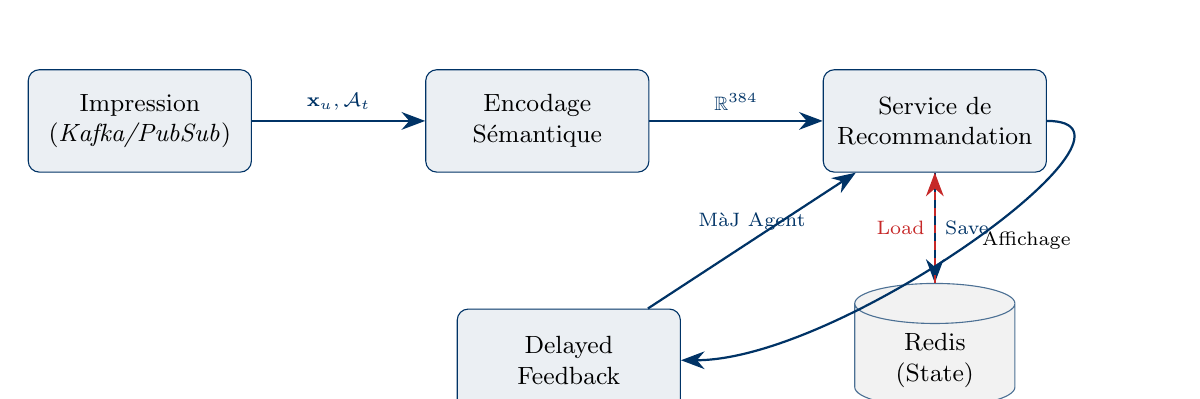
\begin{tikzpicture}[
    node distance=1.4cm and 2.2cm,
    block/.style={rectangle, draw=emiBlue, fill=emiBlue!8, text width=2.6cm,
                  minimum height=1.3cm, align=center, rounded corners=4pt, font=\small},
    db/.style={cylinder, draw=emiBlue!70, fill=gray!10, shape border rotate=90,
               aspect=0.25, text width=1.8cm, minimum height=1.2cm, align=center, font=\small},
    arrow/.style={-{Stealth[length=3mm]}, thick, emiBlue},
    darrow/.style={-{Stealth[length=3mm]}, dashed, thick, emiRed}
]
    \node[block] (imp)      {Impression\\(\textit{Kafka/PubSub})};
    \node[block, right=of imp]  (enc)  {Encodage\\Sémantique};
    \node[block, right=of enc]  (api)  {Service de\\Recommandation};
    \node[db,    below=of api]  (red)  {Redis\\(State)};
    \node[block, left=of red]   (fb)   {Delayed\\Feedback};

    \draw[arrow] (imp) -- node[above,font=\scriptsize]{$\mathbf{x}_u,\mathcal{A}_t$} (enc);
    \draw[arrow] (enc) -- node[above,font=\scriptsize]{$\mathbb{R}^{384}$} (api);
    \draw[arrow] (api) -- node[right,font=\scriptsize]{Save} (red);
    \draw[darrow] (red) -- node[left,font=\scriptsize]{Load} (api);
    \draw[arrow] (api) .. controls +(right:3cm) and +(right:3.5cm) ..
                 node[right,font=\scriptsize,text=black]{Affichage} (fb);
    \draw[arrow] (fb)  -- node[above,font=\scriptsize]{MàJ Agent} (api);
\end{tikzpicture}
}
\caption{Architecture fonctionnelle de la boucle de décision (\textit{Closed-Loop}).}
\label{fig:closed_loop_ch4}
\end{figure}

Le flux de données suit cinq étapes : (1) capture de l'impression, (2) encodage sémantique via SentenceTransformer \parencite{reimers2019sentence}, (3) sélection par H-DeepBandit × $\varepsilon$-Constraint \parencite{riquelme2018deep,ehrgott2005multicriteria}, (4) collecte du feedback, (5) mise à jour continue du modèle.

\subsection{Le Cœur de Décision : RecommendationService}

La classe \texttt{RecommendationService} orchestre toute la logique de décision. Elle encapsule :

\begin{itemize}
    \item L'\textbf{encodeur sémantique} : \texttt{all-MiniLM-L6-v2} \parencite{reimers2019sentence} ($\mathbb{R}^{384}$).
    \item L'\textbf{agent H-DeepBandit} : ensemble de 5 MLP ($768 \to 128 \to 64 \to 1$), deux têtes (engagement, revenue).
    \item Le \textbf{registre d'annonces} : ajout dynamique via \texttt{expand\_arms()} (zero-shot).
    \item La \textbf{politique MOO} : $\varepsilon$-Constraint maximisant le CTR sous contrainte de revenue.
\end{itemize}

\begin{listing}[htbp]
\begin{minted}[frame=lines, framesep=2mm, bgcolor=gray!8, fontsize=\footnotesize, breaklines]{python}
def recommend(self, user_text: str, available_ads: List[AdInfo]):
    user_emb = self.encoder.encode(user_text)          # 1. Encodage
    for ad in available_ads:                            # 2. Zero-Shot Cold-Start
        if ad.ad_id not in self.ad_id_to_idx:
            ad_emb = self.encoder.encode(ad.title + " " + ad.description)
            self.agent.expand_arms({ad.ad_id: ad_emb})
    predictions = self.agent.predict_all(context=user_emb)  # 3. Prédiction
    selected_idx = epsilon_constraint_policy(           # 4. Politique MOO
        predictions=predictions, epsilon=self.epsilon)
    return self.idx_to_ad_id[selected_idx]
\end{minted}
\caption{Méthode de recommandation principale (\texttt{RecommendationService}).}
\label{lst:recommend_ch4}
\end{listing}

\subsection{L'API REST (FastAPI)}

L'API expose quatre \textit{endpoints} :

\begin{table}[H]
    \centering
    \begin{tabular}{l l L{7cm}}
        \toprule
        \textbf{Méthode} & \textbf{Endpoint} & \textbf{Description} \\
        \midrule
        POST & \texttt{/recommend} & Sélection de l'annonce optimale \\
        POST & \texttt{/feedback}  & Feedback (clic, conversion, revenue) avec delayed feedback \\
        GET  & \texttt{/metrics}   & Statistiques glissantes (CTR, revenue, latence) \\
        GET  & \texttt{/health}    & Sonde de monitoring Cloud Run / Kubernetes \\
        \bottomrule
    \end{tabular}
    \caption{Endpoints de l'API REST.}
    \label{tab:api_endpoints_ch4}
\end{table}

\subsection{L'Abstraction d'Infrastructure (Factory Pattern)}

Toutes les interactions réseau utilisent le \textit{design pattern Factory} (\texttt{src/infra/factory.py}). Le code métier ne connaît que trois interfaces abstraites : \texttt{MessageProducer}, \texttt{MessageConsumer}, \texttt{StateStore}. La variable d'environnement \texttt{QUEUE\_BACKEND} instancie soit \textbf{Kafka} (développement local), soit \textbf{GCP Pub/Sub} (production).

%------------------------------------------------------------------------
%  4.2 — Delayed Feedback
%------------------------------------------------------------------------
\section{Gestion du \textit{Delayed Feedback} (FALCON)}
\label{sec:delayed_feedback_ch4}

\subsection{Problématique du Biais de Pénalisation}

Si le clic ($O_1$) est immédiat, la conversion ($O_2$) arrive des heures plus tard. Sans mécanisme adapté, le modèle apprend \texttt{revenue = 0} pour toutes les impressions $\to$ \textbf{biais systémique} qui bloque la politique $\varepsilon$-Constraint.

\subsection{Implémentation Inspirée de FALCON}

Inspirée de \parencite{ktena2019addressing}, la solution utilise un champ \texttt{feedback\_type} à trois modes via \texttt{POST /feedback} :

\begin{itemize}
    \item \textbf{\texttt{click}} (immédiat) : mise à jour de la tête engagement uniquement ; impression stockée dans un buffer \textit{pending}.
    \item \textbf{\texttt{conversion}} (asynchrone) : réconciliation avec l'impression d'origine + facteur de correction :
    $$\text{Revenue Corrigé} = \frac{\text{Revenue Effectif}}{\text{Confirm Rate}}, \quad \text{Confirm Rate} = \frac{N_{\text{Total}} - N_{\text{Pending}}}{N_{\text{Total}}}$$
    \item \textbf{\texttt{full}} : clic et revenue disponibles simultanément (simulation).
\end{itemize}

Un processus de \textit{garbage collection} expire automatiquement les impressions en attente depuis plus de 24 heures (seuil d'attribution standard en marketing digital).

%------------------------------------------------------------------------
%  4.3 — Déploiement
%------------------------------------------------------------------------
\section{Architecture de Déploiement Cloud-Native}
\label{sec:deploiement_ch4}

\subsection{Environnement Local (Docker Compose)}

5 conteneurs forment le stack de développement :

\begin{enumerate}
    \item \textbf{API FastAPI} : interface d'inférence temps réel.
    \item \textbf{Consumer Streaming} : worker closed-loop via Kafka.
    \item \textbf{Kafka + Zookeeper} : message broker des événements.
    \item \textbf{Redis} : persistence des poids PyTorch \parencite{paszke2019pytorch} du H-DeepBandit.
    \item \textbf{Grafana} : monitoring des métriques du pipeline.
\end{enumerate}

\subsection{Déploiement Serverless sur GCP (Production)}

\begin{table}[H]
    \centering
    \begin{tabular}{l l l}
        \toprule
        \textbf{Composant} & \textbf{Docker (Local)} & \textbf{GCP (Production)} \\
        \midrule
        Hébergement API   & Uvicorn interne             & \textbf{Cloud Run} (autoscaling $0 \to N$) \\
        Message Broker    & Apache Kafka                & \textbf{Cloud Pub/Sub} \\
        State Store       & Redis Alpine 7              & \textbf{Memorystore} (managed) \\
        CI/CD             & Shell local                 & \textbf{Cloud Build} + Artifact Registry \\
        \bottomrule
    \end{tabular}
    \caption{Mapping de l'infrastructure locale vers GCP.}
    \label{tab:mapping_infra_ch4}
\end{table}

Le déploiement est automatisé via \texttt{deploy/gcp\_deploy.sh} (Infrastructure as Code). Cloud Run permet de descendre à zéro instances (économies lors d'interruptions de trafic) et de scaler exponentiellement lors des pics.

%------------------------------------------------------------------------
%  4.4 — Validation Temps Réel
%------------------------------------------------------------------------
\section{Validation Temps Réel}
\label{sec:validation_temps_reel_ch4}

\subsection{Test d'Intégration End-to-End}

Un test d'intégration en 9 étapes reproduit le cycle de vie complet d'un système publicitaire (de l'initialisation du service au test des endpoints FastAPI), incluant le delayed feedback. \textbf{Résultat : 9/9 réussis}, avec une latence d'inférence mesurée à $\sim 8$~ms.

\subsection{Simulation Temps Réel (500 itérations)}

Une simulation de 500 itérations a été conduite avec 10 profils utilisateurs et 10 annonces, reproduisant les quatre phases du cycle de vie :

\begin{table}[H]
    \centering
    \begin{tabular}{l l L{7cm}}
        \toprule
        \textbf{Phase} & \textbf{Timestep} & \textbf{Description} \\
        \midrule
        Warm-up    & $t = 0 \to 100$   & Apprentissage initial avec 6 annonces \\
        Stable     & $t = 100 \to 300$ & Régime convergé, exploitation sémantique \\
        Cold-Start & $t = 300$          & Injection de 4 nouvelles annonces ($6 \to 10$ bras) \\
        Recovery   & $t = 350 \to 500$ & Adaptation via zero-shot transfer \\
        \bottomrule
    \end{tabular}
    \caption{Phases de la simulation temps réel.}
    \label{tab:phases_sim_ch4}
\end{table}

\subsubsection{Évolution des KPIs}

\begin{figure}[htbp]
    \centering
    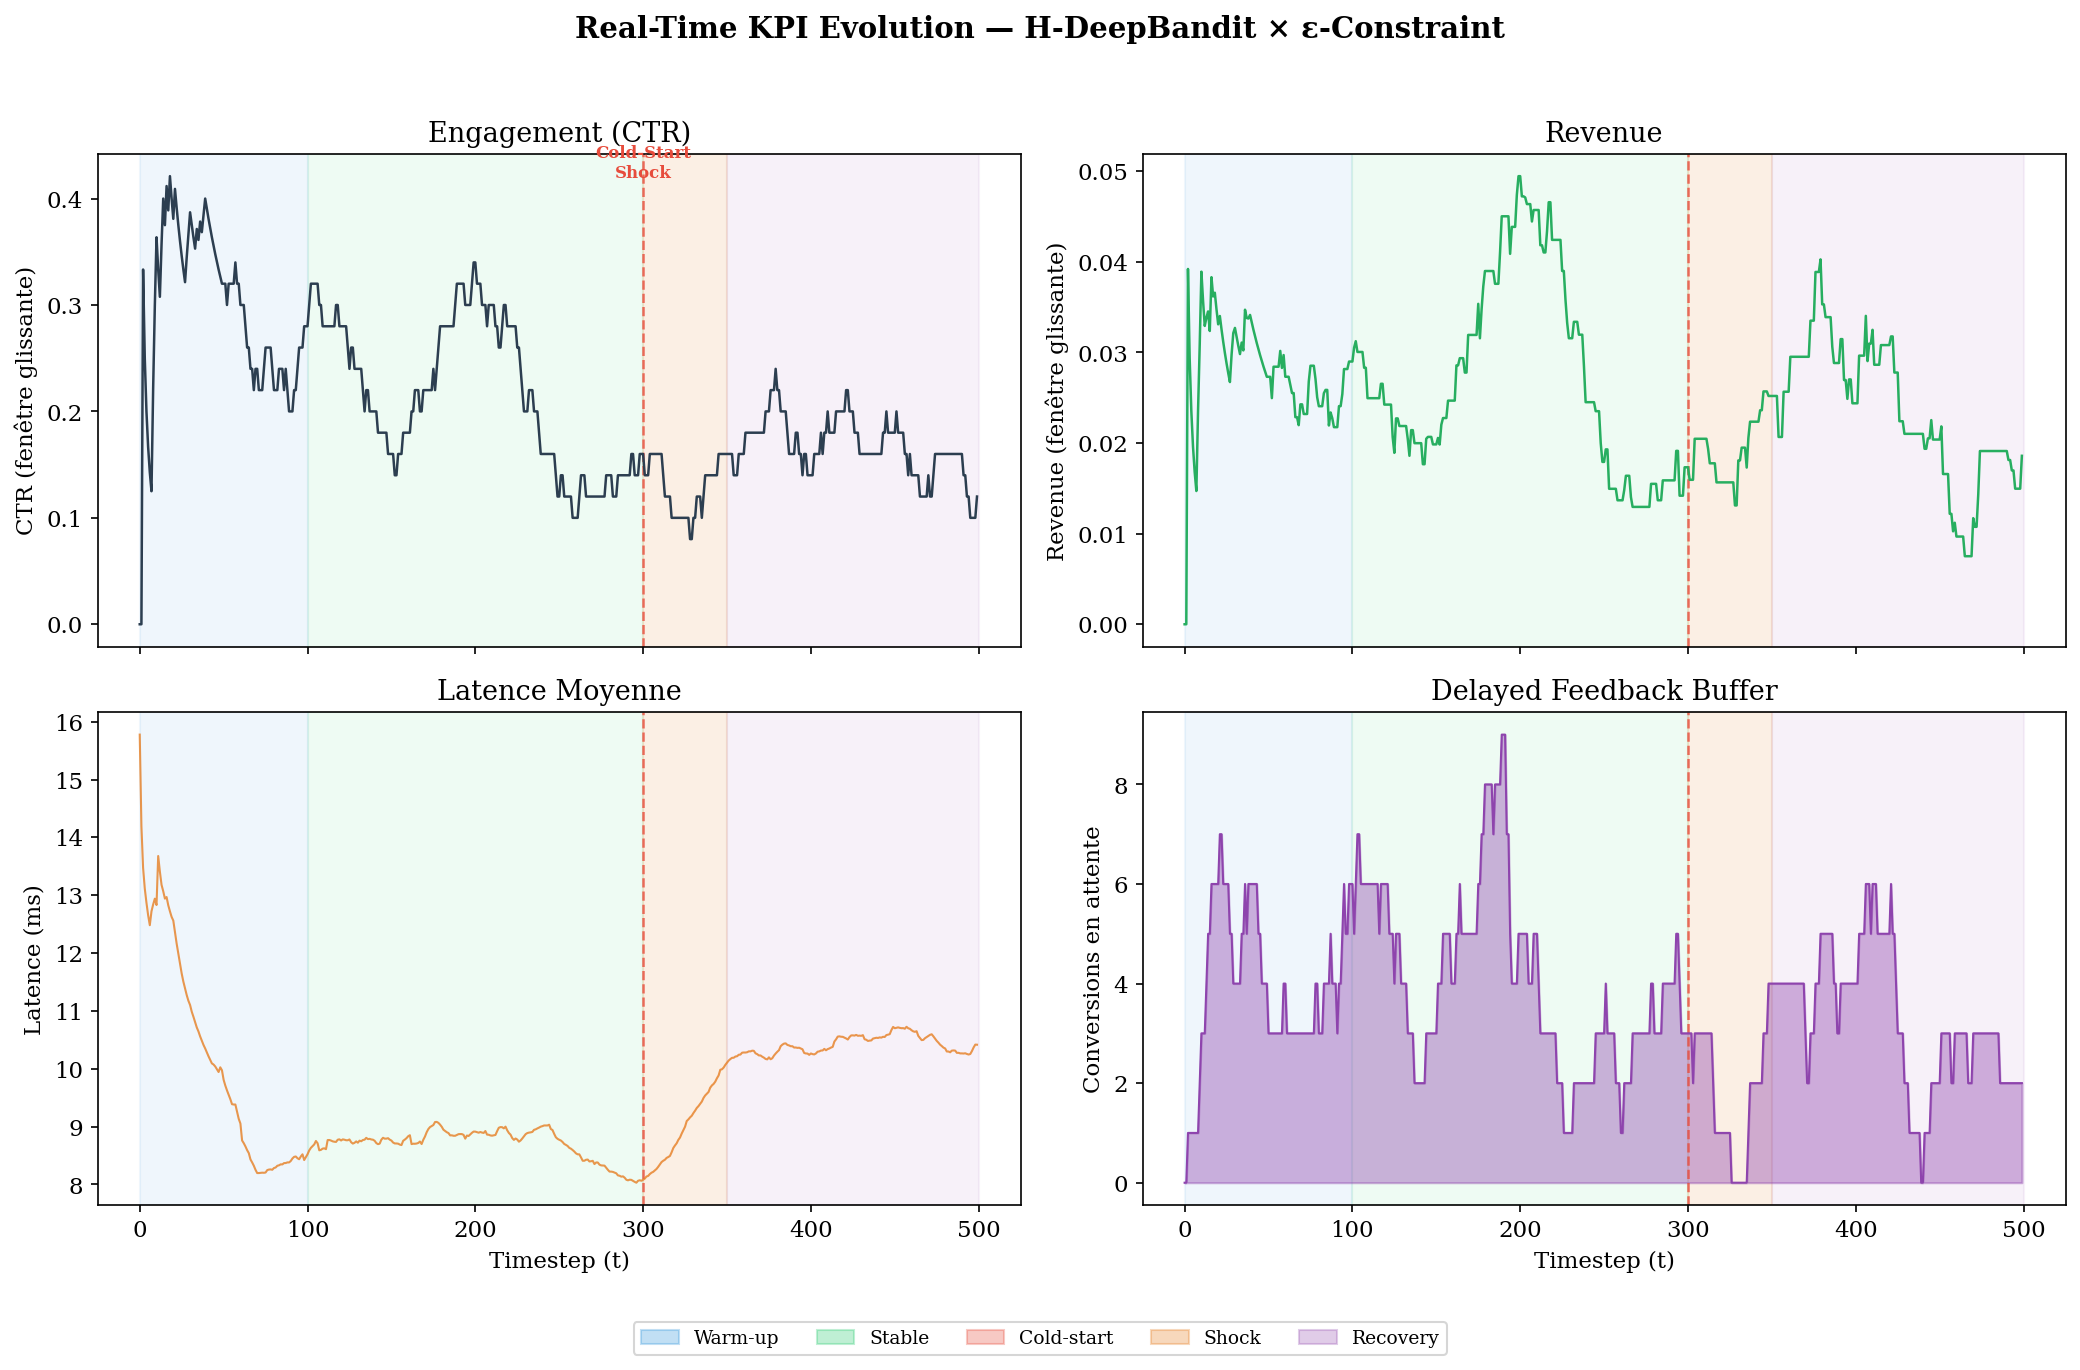
\includegraphics[width=\textwidth]{realtime_kpi_evolution.png}
    \caption{Évolution des KPIs sur 500 itérations : (a) CTR glissant, (b) Revenue glissant, (c) Latence, (d) Conversions en attente (buffer delayed feedback). La ligne verticale indique le cold-start shock à $t=300$.}
    \label{fig:kpi_evolution_ch4}
\end{figure}

\textbf{Observations} :
\begin{itemize}
    \item \textbf{Convergence} : le CTR passe de $\sim 0.08$ (exploration) à $\sim 0.34$ en phase stable.
    \item \textbf{Latence} : $\sim 9$~ms en moyenne, $\sim 10$~ms post cold-start (6 $\to$ 10 bras) --- bien sous le SLA de 50~ms du RTB \parencite{yuan2013real}.
    \item \textbf{Delayed feedback} : le buffer fluctue entre 0 et 8 --- le mécanisme FALCON fonctionne correctement \parencite{ktena2019addressing}.
\end{itemize}

\subsubsection{Résilience au Cold-Start}

\begin{figure}[htbp]
    \centering
    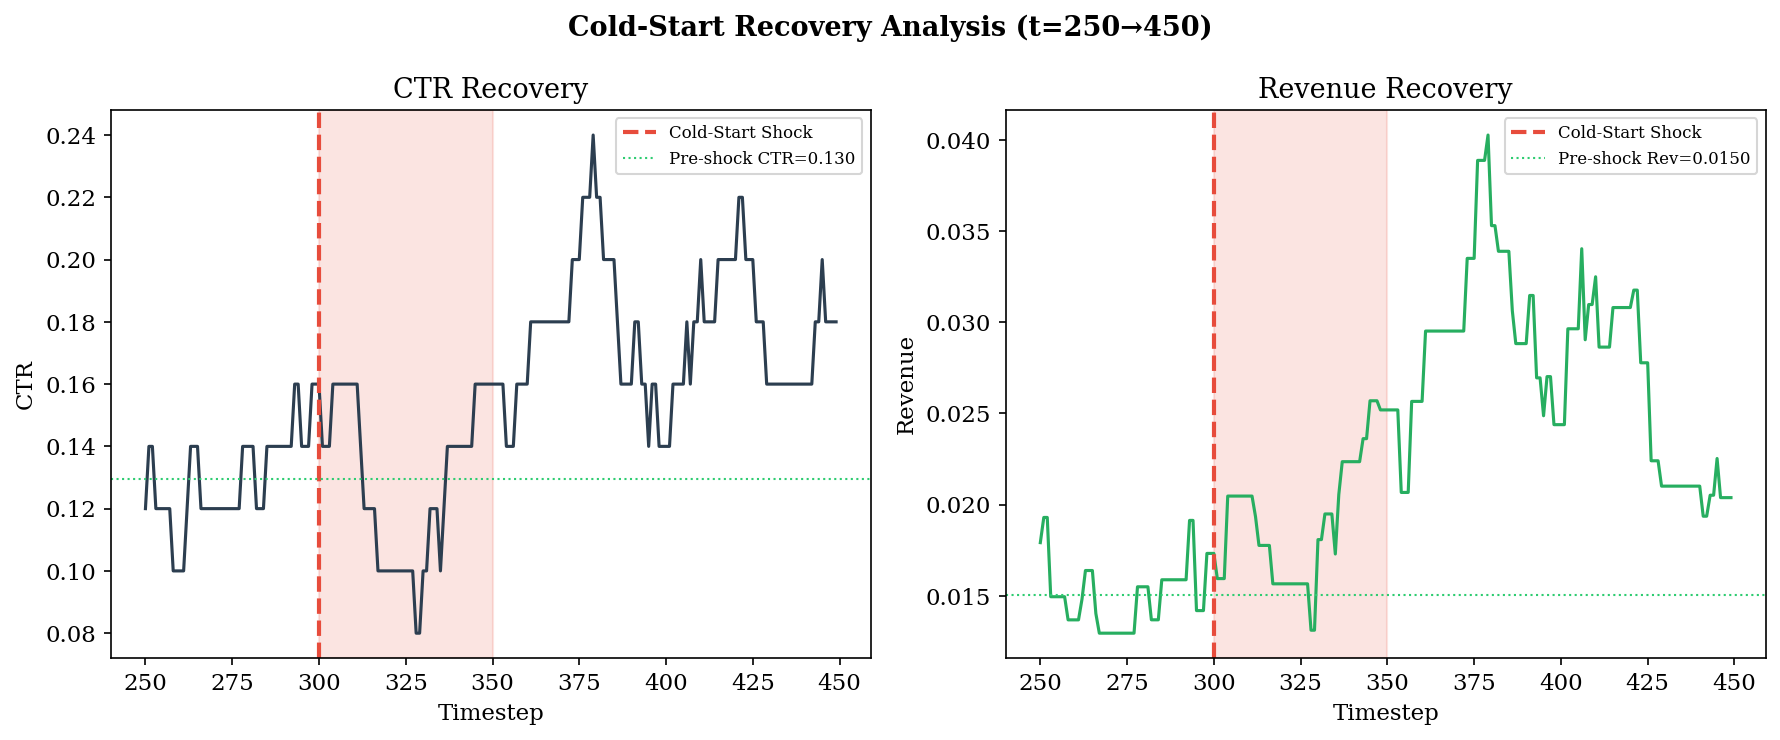
\includegraphics[width=0.85\textwidth]{realtime_cold_start_recovery.png}
    \caption{Zoom sur la récupération post cold-start ($t = 250 \to 450$) : injections de 4 nouvelles annonces absorbées quasi-instantanément grâce au zero-shot transfer.}
    \label{fig:cold_start_ch4}
\end{figure}

\subsubsection{Distribution des Sélections}

\begin{figure}[htbp]
    \centering
    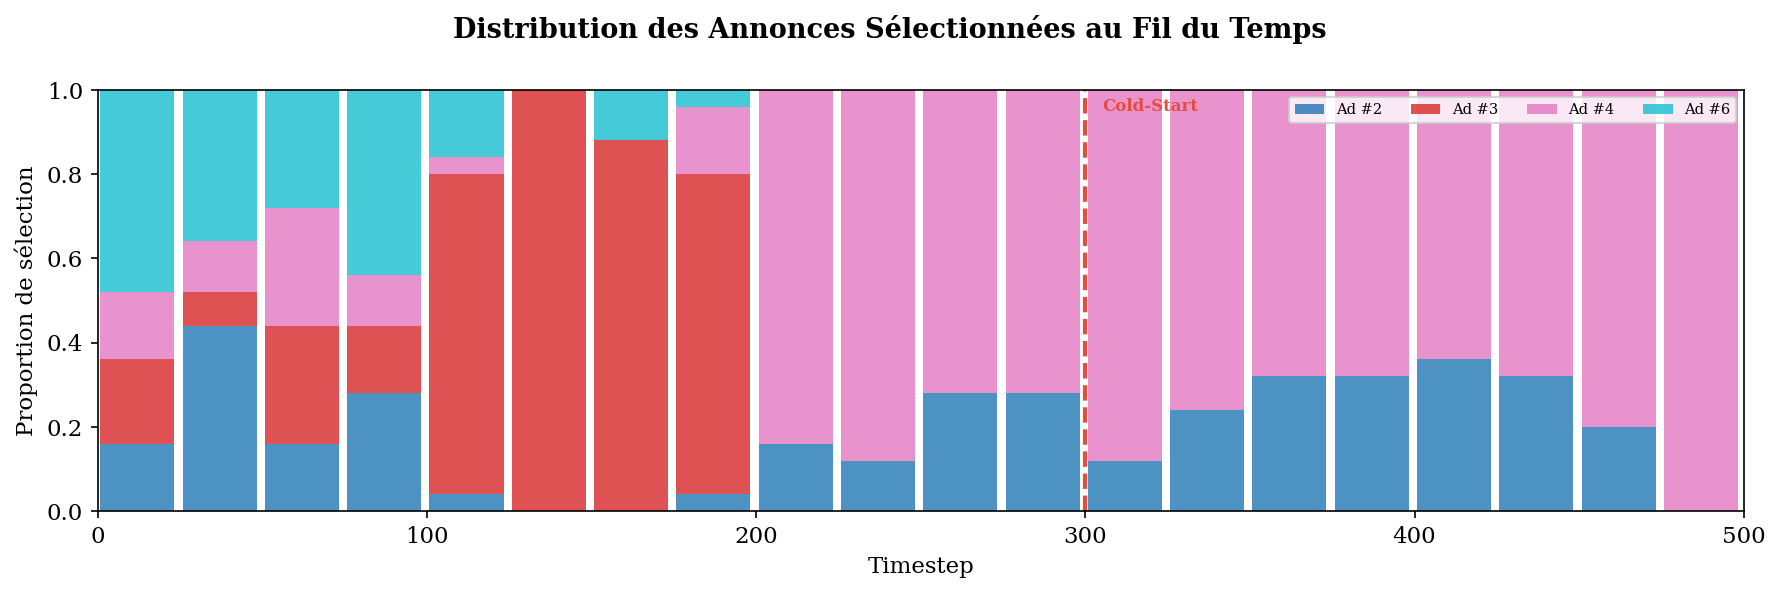
\includegraphics[width=0.85\textwidth]{realtime_arm_distribution.png}
    \caption{Distribution des annonces sélectionnées : le modèle exploite les annonces à haute affinité sémantique tout en maintenant une exploration résiduelle.}
    \label{fig:arm_dist_ch4}
\end{figure}

\subsection{Test de Charge}

\begin{table}[H]
    \centering
    \begin{tabular}{C{1.8cm} C{2cm} C{2cm} C{2cm} C{2cm} C{1.8cm}}
        \toprule
        \textbf{Conc.} & \textbf{Lat. Moy.} & \textbf{P95} & \textbf{P99} & \textbf{RPS} & \textbf{Erreurs} \\
        \midrule
        1  & 11,8~ms   & 19,4~ms   & 21,3~ms   & \textbf{84}  & 0 \\
        5  & 353,9~ms  & 376,2~ms  & 409,9~ms  & 14,1 & 0 \\
        10 & 738,1~ms  & 779,9~ms  & 823,8~ms  & 13,5 & 0 \\
        25 & 1\,778~ms & 1\,886~ms & 1\,907~ms & 13,9 & 0 \\
        50 & 3\,495~ms & 3\,725~ms & 3\,795~ms & 14,0 & 0 \\
        \bottomrule
    \end{tabular}
    \caption{Résultats du test de charge (single-worker Uvicorn).}
    \label{tab:load_test_ch4}
\end{table}

\begin{figure}[htbp]
    \centering
    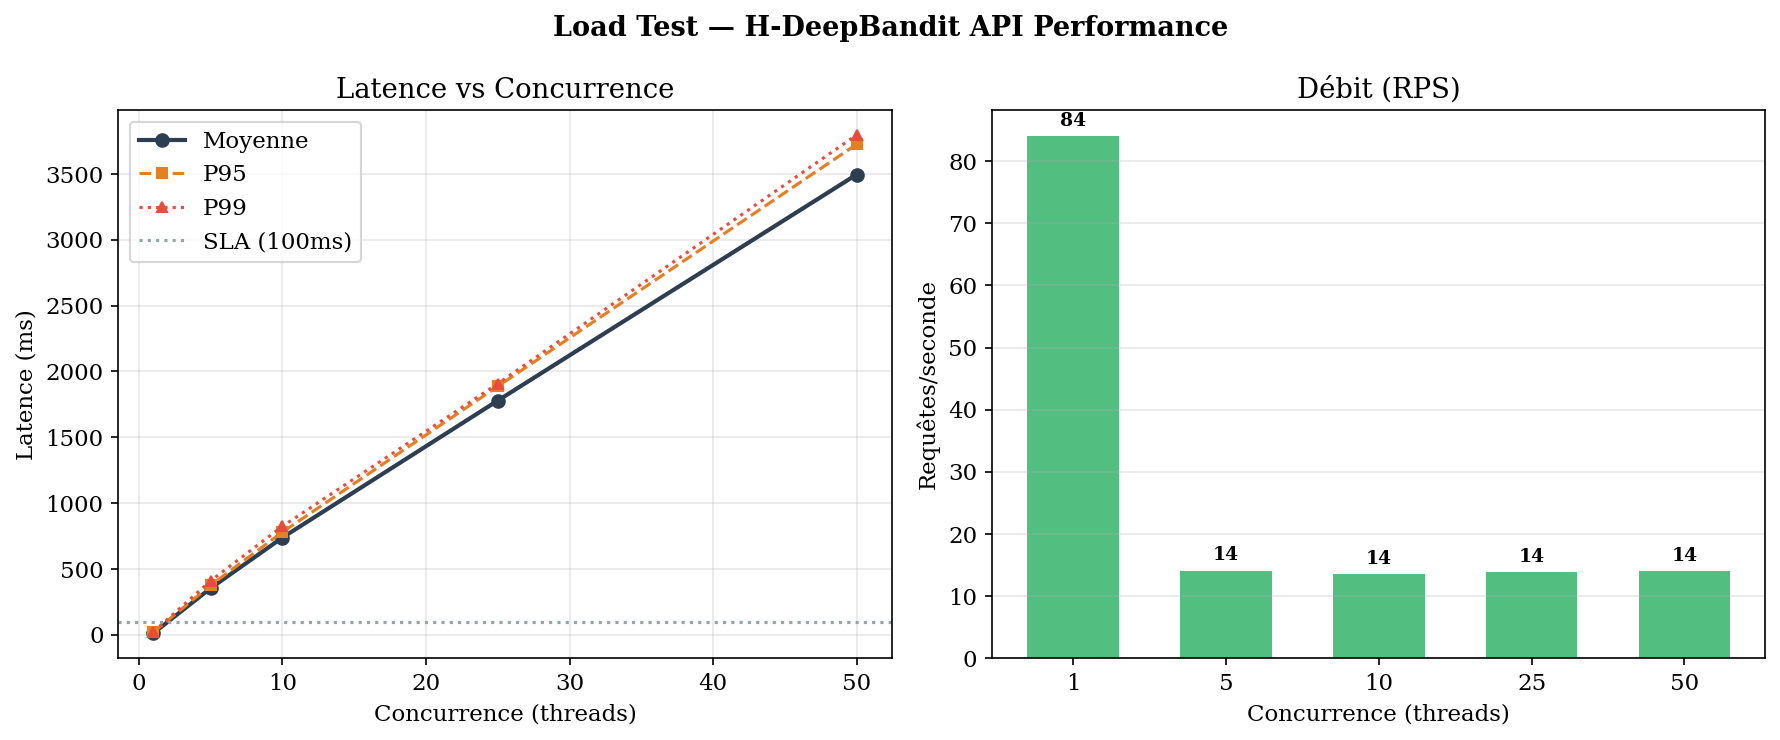
\includegraphics[width=0.85\textwidth]{load_test_latency.png}
    \caption{Latence (moy., P95, P99) et débit (RPS) en fonction de la concurrence.}
    \label{fig:load_test_ch4}
\end{figure}

En mode \textit{single-worker}, le système atteint \textbf{84 req/s} avec une latence P95 de 19,4~ms (concurrence = 1). Le débit se stabilise à $\sim14$~req/s au-delà de 5 threads concurrents (CPU-bound sur SentenceTransformer). En production Cloud Run, le scaling horizontal absorbe la charge totale. \textbf{Zéro erreur} à tous les niveaux de concurrence.

%------------------------------------------------------------------------
%  4.5 — Limites et Perspectives
%------------------------------------------------------------------------
\section{Limites et Perspectives}
\label{sec:limites_ch4}

\begin{enumerate}
    \item \textbf{Données simulées} : validation sur \texttt{SemanticRewardSimulator}; un déploiement sur données Google Ads réelles est nécessaire \parencite{chapelle2014simple}.
    \item \textbf{Single-worker} : le scaling horizontal multi-worker avec état partagé Redis reste à valider.
    \item \textbf{Embeddings figés} : un fine-tuning de \texttt{all-MiniLM-L6-v2} \parencite{reimers2019sentence} sur données publicitaires réelles améliorerait les représentations sémantiques.
    \item \textbf{Google Ads API} : intégration avec le flux réel d'impressions pour une validation en production.
    \item \textbf{Deep RL} : extension vers PPO/SAC avec historique d'états pour capturer les dynamiques séquentielles.
    \item \textbf{A/B Testing} : protocole de test contrôlé pour quantifier le gain business réel chez les clients Devoteam.
\end{enumerate}

%------------------------------------------------------------------------
%  Conclusion du chapitre
%------------------------------------------------------------------------
\section*{Conclusion du Chapitre}
\addcontentsline{toc}{section}{Conclusion du Chapitre}

Ce chapitre a démontré la viabilité du système en conditions temps réel :
\begin{itemize}
    \item Une architecture \textbf{closed-loop} complète (impression $\to$ encodage $\to$ décision $\to$ feedback $\to$ MàJ).
    \item Un mécanisme \textbf{FALCON} garantissant l'intégrité des estimations de revenue malgré les délais de conversion.
    \item Un déploiement \textbf{dual} Docker/GCP via le pattern Factory.
    \item Une \textbf{latence de $\sim9$~ms} et un débit de \textbf{84 req/s}, avec zéro erreur sous charge.
\end{itemize}

Ces résultats valident le passage du prototype de recherche au système opérationnel, clôturant le triptyque \textit{théorie--expérimentation--industrialisation}.

\clearpage

%========================================================================%
%  Conclusion Générale                                                     %
%========================================================================%

\chapter*{Conclusion Générale}
\addcontentsline{toc}{chapter}{Conclusion Générale}

\section*{Synthèse des Contributions}

Ce Projet de Fin d'Études avait pour ambition de concevoir, implémenter et valider un \textbf{Système de Recommandation Publicitaire Multi-Objectif} capable d'opérer en temps réel. Le travail réalisé couvre l'ensemble du spectre théorie--expérimentation--industrialisation.

\textbf{Chapitre 1} a posé le cadre général : écosystème publicitaire digital, systèmes de recommandation, et mécanisme du RTB. La problématique centrale a été formalisée --- optimiser simultanément l'engagement (CTR) et le revenu (eCPM) sous les contraintes temporelles du Real-Time Bidding.

\textbf{Chapitre 2} a établi le cadre théorique : formalisation MOIP \parencite{deb2001multi}, état de l'art des agents bandits \parencite{li2010contextual, riquelme2018deep} et des politiques MOO \parencite{deb2002fast,ehrgott2005multicriteria}. L'approche hybride sémantique a été proposée, fondée sur l'encodage SentenceTransformer \parencite{reimers2019sentence} et le modèle global partagé.

\textbf{Chapitre 3} a validé l'approche via un benchmark exhaustif de \textbf{142 configurations}. Le champion identifié --- \textbf{H-DeepBandit $\times$ $\varepsilon$-Constraint} --- est le seul point conjoint $(0.663,\ 0.094)$ dominant strictement son homologue classique sur les deux objectifs simultanément. Le transfert zéro-shot démontre un avantage de $+0.132$ en engagement face au cold-start.

\textbf{Chapitre 4} a traduit ce modèle en un système opérationnel : architecture closed-loop, gestion du delayed feedback (FALCON \parencite{ktena2019addressing}), déploiement cloud-native (Docker / GCP Cloud Run). La validation confirme une latence de $\sim 9$~ms, un débit de 84~req/s, et zéro erreur sous charge.

\section*{Apport pour Devoteam Maroc}

Ce projet livre à Devoteam un \textbf{accélérateur technologique} réutilisable pour ses clients :

\begin{itemize}
    \item Une architecture \textbf{cloud-native} (Docker $\to$ GCP) via le pattern Factory.
    \item Un système \textbf{auto-adaptatif} qui apprend en continu sans re-entraînement offline.
    \item Un \textbf{framework de benchmark} (142 configurations) permettant d'évaluer objectivement tout nouvel agent ou politique.
\end{itemize}

\section*{Perspectives}

\begin{enumerate}
    \item \textbf{Intégration Google Ads API} : validation en conditions de production réelles.
    \item \textbf{Deep Reinforcement Learning} : exploration des architectures PPO/SAC avec historique d'états.
    \item \textbf{A/B Testing} : quantification du gain business réel par rapport aux politiques existantes.
    \item \textbf{Multi-tenant} : adaptation de l'architecture pour servir plusieurs clients simultanément.
    \item \textbf{Fine-tuning des embeddings} : spécialisation de \texttt{all-MiniLM-L6-v2} sur des données publicitaires réelles.
\end{enumerate}

\clearpage

%--- Bibliographie ---
\printbibliography[heading=bibintoc, title={Références Bibliographiques}]

\end{document}
